\chapter{Data Analysis and Preprocessing}\label{chap:data}

Our dataset comprises approximately 400 sessions obtained from 80 distinct
patients. These sessions, recorded at irregular intervals, incorporate a 3D
scan of the patient and a multitude of other measurements such as weight,
height, body fat percentage, and more.

\begin{table}[h]
    \centering
    \begin{tabular}{c c l c}
        \toprule
        Type                               & Source                                                                                         & Measurement (unit)                        \\
        \midrule
        \multirow{3}{*}{Anthropometric}    & \multirow{3}{4cm}{flexible measuring tape}                                                     & Wrist (cm)                                \\
                                           &                                                                                                & Waist (cm)                                \\
                                           &                                                                                                & Hip (cm)                                  \\
        \midrule

        \multirow{6}{*}{Body composition}  & \multirow{6}{4cm}{Tanita\textregistered\ MC 780-P MA and Seca\textregistered\ 213 stadiometer} & Fat per limb and trunk (\%)               \\
                                           &                                                                                                & Muscle per limb and trunk (\%)            \\
                                           &                                                                                                & Total fat and muscle (\%)                 \\
                                           &                                                                                                & Visceral fat area (cm\textsuperscript{2}) \\
                                           &                                                                                                & Weight (kg)                               \\
                                           &                                                                                                & Height (m)                                \\
        \midrule

        \multirow{3}{*}{Other, Lifestyle}  & \multirow{3}{4cm}{Interview}                                                                   & Activity   (score)                        \\
                                           &                                                                                                & Gender                                    \\
                                           &                                                                                                & Age (years)                               \\

        \midrule

        \multirow{3}{*}{Blood (capillary)} & \multirow{3}{4cm}{Accutrend\textregistered\ Plus}                                              & Glucose (mg/dL)                           \\
                                           &                                                                                                & Cholesterol (mg/dL)                       \\
                                           &                                                                                                & Triglycerides (mg/dL)                     \\

        \midrule

        \multirow{2}{*}{Blood pressure}    & \multirow{2}{4cm}{Omron\textregistered\ M3}                                                    & Systolic pressure (mmHg)                  \\
                                           &

                                           & Diastolic pressure (mmHg)                                                                                                                  \\
        \bottomrule

    \end{tabular}
    \caption{Measurements collected from each session.}
\end{table}

\todo[]{${https://rua.ua.es/dspace/bitstream/10045/124160/6/Garcia-dUrso_etal_2022_IEEEAccess.pdf}$}
The raw data, however, required extensive cleaning before it could be analyzed. We encountered sessions missing certain measurements and numerous data outliers. After our data cleaning process, we were left with approximately 200 viable sessions.

\begin{figure}[h]
    \centering
    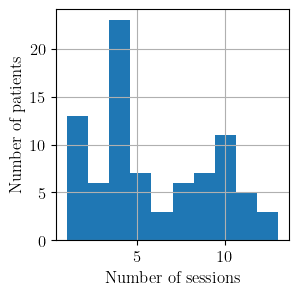
\includegraphics[width=0.5\textwidth]{files/sessions_per_patient}
    \caption{Variation in the number of sessions per patient}
    \label{fig:sessions-per-patient}
\end{figure}

As Figure~\ref{fig:sessions-per-patient} illustrates, the number of sessions
per patient varied significantly, with some patients attending only a single
session and others attending over ten. Given that neural networks necessitate
uniform input shapes, we were faced with a challenge. We'll elaborate on how we
tackled this problem in Chapter \ref{chap:nn}.
\subsection{Data Cleaning and Outlier Detection}

A data cleaning pipeline was constructed utilizing the \gls{pandas} library.
Essential steps encompassed missing data treatment, duplicate removal, and
variable unit standardization.

We indexed our dataset with a multi-index that included the patient's id and
the session number. This system facilitated patient-specific data iteration and
simplified the process of pinpointing patient data discrepancies.

Upon scrutinizing plotted data, we discovered that the decimal separator was a
common source of errors. Many measurements appeared to be inflated by a factor
of 10, prompting us to devise tailored rules to correct this. Additional rules
were implemented to identify and discard out-of-range values or those
conflicting with other measurements. These rules included:

\begin{itemize}
    \item Small variation between measurements of different limbs, such as muscle or fat
          percentage discrepancies between left and right arms.
    \item Ensuring that the combined muscle and fat percentages do not exceed 100%.
    \item Verifying that the fat and muscle percentage levels individually stay below 100%—values exceeding this typically indicate a measurement inflated by a factor of 10.
\end{itemize}

Despite these rectifications, some outliers persisted. We experimented with a
system that flagged dramatic session-to-session changes, but found it too
susceptible to false positives. Eventually, we opted to manually inspect the
data, flagging conspicuous outliers for removal.

\begin{figure}[h]
    \centering
    \begin{subfigure}{\textwidth}
        \centering
        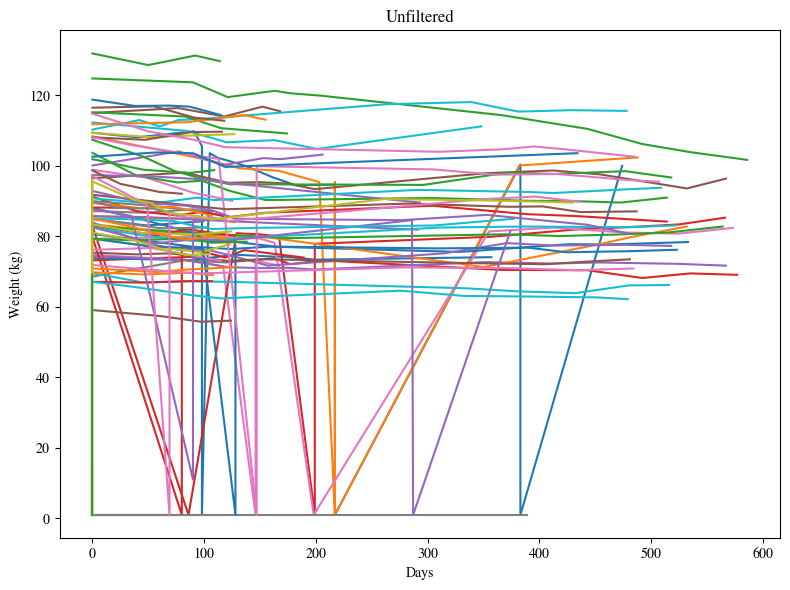
\includegraphics[width=0.8\textwidth]{files/weight_unfiltered}
        \caption{Raw weight}
    \end{subfigure}
    \begin{subfigure}{\textwidth}
        \centering
        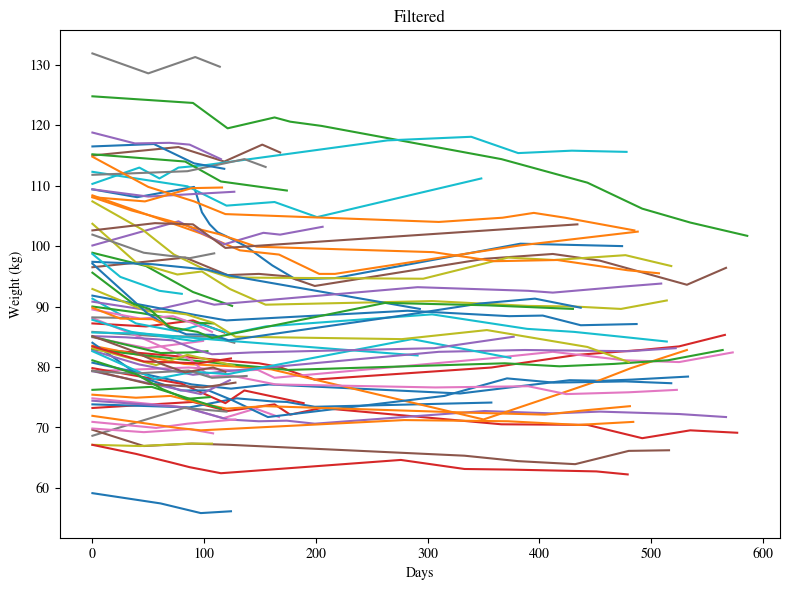
\includegraphics[width=0.8\textwidth]{files/weight_filtered}
        \caption{Filtered weight}
    \end{subfigure}
    \caption{Weight measurements pre and post filtering}
\end{figure}
\section{SMPL for Body Representation}

In order to represent the body shape we opted to use \gls{smpl}. \gls{smpl}
encodes the body shape and pose using a low-dimensional linear space. The body
shape is encoded using 10 shape parameters ($\beta$), and the pose is encoded
using 72 pose parameters ($\theta$). As our interest lies in body shape, we
employed only the shape parameters.

We extracted \gls{smpl} parameters --- shape ($\beta$) and pose ($\theta$) ---
from the 3D scans using a custom minimization algorithm. This procedure
consisted of:

\begin{itemize}
    \item Acquiring and Preprocessing of 3D Data: The Tech4Diet project's system, fitted
          with 13 Intel RealSense RGB-D cameras, was used to capture the 3D data. This
          data was then preprocessed to minimize noise and optimize 3D scan alignment.

    \item Estimating an Intermediate Template using a BPS Neural Network: The \gls{bps}
          method was used to generate an intermediate 3D model by encoding a set of
          points into fixed-distance representations. A DenseNet neural network then took
          this \gls{bps} representation as input to predict the vertex positions of a
          template resembling the input point cloud.

    \item First Minimization: \gls{bps} to \gls{smpl}: We minimized the pose and shape
          parameters of the \gls{smpl} model to align it with the template created by the
          \gls{bps}.

    \item Second Minimization: 3D Scan to \gls{smpl}: A second minimization was performed
          to align the \gls{smpl} model with the 3D scan from the RGB-D sensors. We
          proposed an algorithm to enhance the speed and accuracy of this process by
          segmenting the model into body parts, applying rigid registration, and then
          using a custom minimization function that considered both distance and normal
          angles.
\end{itemize}\todo{cite soco2023 nahuel}

Figure~\ref{fig:beta-vis} demonstrates the effects of shape parameter
variations. Although we employed a scale of 3 to amplify their effects for
visualization, actual values are significantly lower. $\beta_0$ regulates the
overall body height, while $\beta_1$ is highly correlated with the body mass
index.

\begin{table}[h]
    \centering
    \begin{tabular}{c | c c c c c c c c c c}
        \toprule
             & $\beta_1$ & $\beta_2$ & $\beta_3$ & $\beta_4$ & $\beta_5$ & $\beta_6$ & $\beta_7$ & $\beta_8$ & $\beta_9$ & $\beta_{10}$ \\
        \midrule
        mean & 0.88      & -0.73     & 0.34      & 0.01      & 0.06      & 0.06      & 0.11      & 0.02      & 0.01      & 0.11         \\

        std  & 0.97      & 0.78      & 0.26      & 0.21      & 0.12      & 0.13      & 0.08      & 0.03      & 0.03      & 0.08         \\

        min  & -1.42     & -2.57     & -0.64     & -0.65     & -0.23     & -0.25     & -0.14     & -0.07     & -0.08     &
        -0.17                                                                                                                           \\

        25\% & 0.12      & -1.26     & 0.15      & -0.14     & -0.01     & -0.02     & 0.04      & 0.00      & -0.01     & 0.06         \\

        50\% & 0.94      & -0.69     & 0.36      & 0.03      & 0.04      & 0.02      & 0.11      & 0.02      & 0.01      & 0.11         \\

        75\% & 1.66      & -0.20     & 0.52      & 0.17      & 0.14      & 0.14      & 0.16      & 0.04      & 0.04      & 0.17         \\

        max  & 2.90      & 2.96      & 0.97      & 0.45      & 0.39      & 0.47      & 0.36      & 0.13      & 0.16      & 0.30         \\
        \bottomrule
    \end{tabular}
    \caption{Statistics of the shape parameters}
\end{table}

\section{Exploring Additional Datasets}

The pursuit of diverse, informative, and applicable data sources is a
significant undertaking when aiming to enhance model performance. In our case,
the quest for additional data proved to be notably challenging due to several
factors.

Firstly, the majority of medical data sets are not readily accessible to the
public. Their inaccessibility is primarily due to privacy and confidentiality
concerns, which are paramount in the realm of medical and health data. The
restrictions on these datasets not only limit their availability but also
obscure their potential usefulness for our research. Without the opportunity to
delve into the contents of these datasets, determining their relevance and
applicability to our work becomes a considerable hurdle.

Secondly, while open-source datasets featuring 3D scans of individuals exist,
they often lack the dynamic quality crucial to our study. Specifically, these
datasets tend to offer static, one-time captures of an individual's physique,
without capturing the temporal changes in body composition. Thus, such datasets
are ill-suited for our purposes since they lack the capability to portray the
progression or regression of an individual's body shape over time — a vital
element for our research into tracking the effects of dietary interventions.

Moreover, we explored datasets not explicitly designed for body composition
study but still containing potentially relevant data, such as datasets from
sports science or anthropometry. However, the limitations in scope, data
granularity, and the lack of consistent body composition measurements made
these datasets inadequate for our purposes.

Upon careful consideration of these challenges, we chose to rely solely on our
proprietary data for model training and evaluation. However, to mitigate the
limitations of our data, we implemented data augmentation techniques designed
to enhance and diversify our dataset artificially. We will delve into the
specifics of these strategies in Chapter \ref{chap:nn}.